\section{HARP extension for flexible performance-complexity balancing}\label{sec:our-method}

While the prolongation used by HARP is sufficient when used only as a means of pre-training, the approach is far too crude when studying the relationship between graph complexity and the quality of graph embedding. In order to overcome this limitation, we present the adaptive prolongation approach. This algorithm works with the pre-coarsened graphs produced by HARP, however, the embedding is learned in a different manner. The \( L \) coarsening steps are decoupled from \( K \) prolongation steps, where \( K \) is independent of \( L \). The prolongation steps are driven by local properties of the graph with relation to the downstream task, allowing for different levels of granularity in different parts of the graph. Let us denote \( \Psi_K, \dots, \Psi_0 \) the resulting embedding sequence. The algorithm starts with the coarsest graph \( G_L \), trains a graph model to compute its embedding \( \Psi_K \) and gradually refines it until reaching the embedding \( \Psi_0 \). These prolongation steps are interlaid with continued training of the graph model, as in standard HARP. A description of a single prolongation step from \( \Psi_{i + 1} \) to \( \Psi_i \) is schematically outlined in Figure~\ref{fig:adaptive-prolongation} and described in more detail in Appendix \ref{sec:app:prolongation-step}.

\begin{figure}
  \centering
  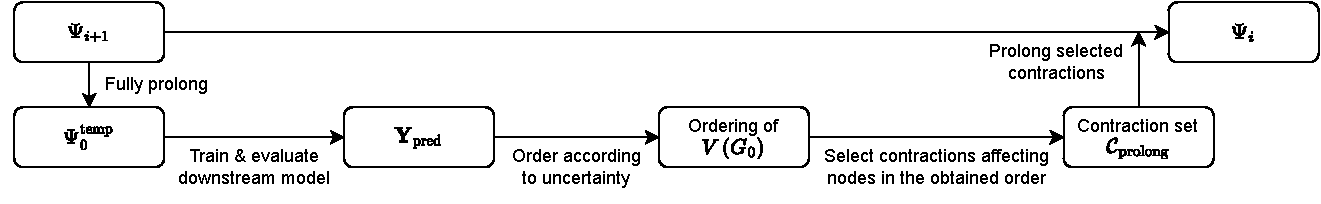
\includegraphics[width=\textwidth]{images/adaptive-prolongation/adaptive-prolongation.pdf}
  \caption{A schematic explanation of the adaptive prolongation algorithm for obtaining the embedding \( \Psi_{i} \) from \( \Psi_{i + 1} \).}
  \label{fig:adaptive-prolongation}
\end{figure}
